\documentclass[11pt]{article}

% Packages
\usepackage[utf8]{inputenc}
\usepackage[T1]{fontenc}
\usepackage{amsmath, amssymb, amsthm}
\usepackage{graphicx}
\usepackage{booktabs}
\usepackage{hyperref}
\usepackage{cleveref}
\usepackage{xcolor}
\usepackage{enumitem}
\usepackage{algorithm}
\usepackage{algorithmic}
\usepackage{multirow}
\usepackage{geometry}
\usepackage{natbib}
\usepackage{microtype}

\geometry{margin=1in}

% Theorem environments
\newtheorem{theorem}{Theorem}
\newtheorem{lemma}{Lemma}
\newtheorem{proposition}{Proposition}
\newtheorem{definition}{Definition}
\newtheorem{remark}{Remark}

% Custom commands
\newcommand{\Fp}{\mathbb{F}_p}
\newcommand{\Fps}{\mathbb{F}_p^*}
\newcommand{\Z}{\mathbb{Z}}
\newcommand{\R}{\mathbb{R}}
\newcommand{\Tmem}{T_{\mathrm{mem}}}
\newcommand{\Tgrok}{T_{\mathrm{grok}}}
\newcommand{\Tfifty}{T_{50}}
\newcommand{\Tninety}{T_{90}}
\newcommand{\Tninfive}{T_{95}}
\newcommand{\Tnine}{T_{99}}
\newcommand{\Gdelay}{G}
\newcommand{\wdmax}{\mathrm{wd}_{\max}}
\newcommand{\Pcore}{P_{\mathrm{core}}}
\newcommand{\Ptotal}{P_{\mathrm{total}}}
\newcommand{\dmodel}{d_{\mathrm{model}}}
\newcommand{\nheads}{n_{\mathrm{heads}}}
\newcommand{\nlayers}{n_{\mathrm{layers}}}

% Title
\title{Grokking the Discrete Logarithm: \\
Scaling Laws and Mechanistic Analysis of \\
Transformer Learning on $\Fps$}

\author{
David Svensson \\
\texttt{david@vesterlund.se} \\
WestCode AI Research
}

\date{}

\begin{document}

\maketitle

\begin{abstract}
We demonstrate that small transformer models \emph{grok} the finite-field discrete logarithm problem (DLP) over $\Fps$ for $p = 113$, achieving 99.8\% test accuracy after a prolonged memorization phase. This is the first systematic study of grokking on the DLP---a problem believed to be cryptographically hard---complementing prior work on modular addition and multiplication. We identify a five-phase training dynamics (initialization, memorization, plateau, circuit formation, cleanup) driven by a progressive weight decay schedule, and show that \emph{slingshot events}---cyclic train-accuracy collapses induced by adaptive optimizers---play a critical role in triggering the grokking transition. We provide a mechanistic analysis via group-structure probes and Fourier spectral analysis on both multiplicative and additive character bases, revealing that the model discovers the cyclic group structure of $\Fps$ and develops sparse representations in the multiplicative character basis. We present a model-size scaling sweep from 90k to 14.4M parameters on LUMI-G, revealing a non-monotonic \emph{grokking valley} where intermediate model sizes fail to grok at fixed training fraction---though we show this valley is train-fraction dependent, not a fundamental capacity barrier. We show that explicitly providing the Chinese Remainder Theorem decomposition of the group order accelerates grokking by $>24\times$, but---surprisingly---a scrambled (randomly permuted) representation groks even faster (verified across 5 seeds), suggesting that information content, not algebraic labeling, drives the acceleration. We measure the critical training fraction for CRT-BOTH grokking (10--15\%) and show that M12 with CRT-BOTH groks primes up to $p = 337$ in $<$8K epochs, with grokking time \emph{decreasing} with prime size. We further demonstrate grokking on prime-order DLP (order-113 subgroup of $\F_{227}^*$), confirming that smooth factorization of the group order is not required, and that the learned algorithm transfers across generators (OOD generalization).
\end{abstract}


% ============================================================================
% 1. INTRODUCTION
% ============================================================================

\section{Introduction}
\label{sec:intro}

The \emph{grokking} phenomenon \citep{power2022grokking}---in which a neural network abruptly transitions from memorization to generalization long after overfitting---has emerged as a powerful lens for studying representation learning in deep neural networks. While initially observed on modular arithmetic tasks (addition, multiplication, permutation composition), the phenomenon has since been studied extensively through the lens of mechanistic interpretability \citep{nanda2023progress}, effective theories of representation learning \citep{liu2022understanding}, circuit efficiency \citep{varma2023explaining}, and the slingshot mechanism \citep{thilak2022slingshot}.

Prior work has primarily focused on operations that are \emph{computationally easy}: modular addition ($a + b \bmod p$) admits an $O(1)$ algorithm via lookup, and modular multiplication ($a \cdot b \bmod p$) similarly has efficient solutions. The discrete logarithm problem (DLP)---given a generator $g$ of $\Fps$ and an element $h \in \Fps$, find $x$ such that $g^x \equiv h \pmod{p}$---is fundamentally different: it is believed to be computationally hard and forms the basis of numerous cryptographic protocols \citep{diffie1976new}. The question of whether neural networks can grok the DLP is thus both scientifically intriguing and cryptographically relevant.

\citet{takhanov2024intractability} showed that gradient-based methods provably cannot efficiently learn the parity bit of the discrete logarithm in cyclic groups of prime order, suggesting fundamental barriers. However, their analysis applies to the \emph{parity bit} (a single bit of the discrete log) rather than the full discrete log mapping, and their hardness result depends on the group order growing large. For small primes ($p = 113$), the full solution space is finite ($|\Fps| = 112$), and the question becomes whether a transformer can discover the group-theoretic structure that enables generalization.

In this work, we make the following contributions:

\begin{enumerate}[leftmargin=*]
    \item \textbf{DLP grokking discovery}: We show that a 2-layer transformer with 427k parameters groks the DLP at $p = 113$, achieving 99.8\% test accuracy after 37k epochs of training with a progressive weight decay schedule (\Cref{sec:discovery}).
    
    \item \textbf{Five-phase training dynamics}: We identify a five-phase training dynamics---initialization, memorization, WD ramp, circuit formation, and cleanup---and show that slingshot events \citep{thilak2022slingshot} play a critical role in triggering the grokking transition (\Cref{sec:dynamics}).
    
    \item \textbf{Mechanistic analysis}: We provide group-structure probes showing the model discovers the cyclic group structure of $\Fps$, and Fourier spectral analysis on both multiplicative and additive character bases, connecting to the ``Discrete-Log Clock'' framework of \citet{doshi2024discrete} (\Cref{sec:mechanistic}).
    
    \item \textbf{Capacity scaling and grokking valley}: We present a scaling sweep from 90k to 14.4M parameters on LUMI-G, revealing a non-monotonic grokking valley where intermediate model sizes fail to grok at fixed training fraction (\Cref{sec:scaling}).
    
    \item \textbf{CRT representation acceleration}: We show that explicitly providing the CRT decomposition accelerates grokking by $>24\times$, but a scrambled representation groks even faster (5 seeds), revealing that information content---not algebraic labeling---drives the acceleration (\Cref{sec:crt}).
    
    \item \textbf{CRT-BOTH scaling}: We show that CRT-BOTH grokking scales to larger primes ($p = 337$) with M12, with grokking time \emph{decreasing} with prime size, and that even M04 (427k params) can grok $p = 241$ in 200 epochs locally (\Cref{sec:m12_crt_scaling,sec:local_crt_scaling}).
    
    \item \textbf{Prime-order DLP and OOD transfer}: We demonstrate grokking on prime-order DLP (no smooth factorization) and show that the learned algorithm transfers across generators (\Cref{sec:prime_order}).
\end{enumerate}


% ============================================================================
% 2. BACKGROUND
% ============================================================================

\section{Background}
\label{sec:background}

\subsection{Grokking and Delayed Generalization}

Grokking was introduced by \citet{power2022grokking}, who observed that neural networks trained on small algorithmic datasets (modular arithmetic, permutation groups) can transition from random-chance test accuracy to perfect generalization after a prolonged period of overfitting. The phenomenon is characterized by three key observations: (1) training accuracy reaches 100\% early in training, (2) test accuracy remains at chance for a long period, and (3) test accuracy abruptly rises to near-perfect levels. The delay between memorization and generalization---the \emph{grokking delay} $\Gdelay = \Tgrok / \Tmem$---can be orders of magnitude.

Several theories have been proposed to explain grokking. \citet{liu2022understanding} presented an effective theory showing that generalization originates from structured representations, with a ``Goldilocks zone'' between memorization and confusion. \citet{nanda2023progress} fully reverse-engineered the algorithm learned by transformers on modular addition, showing it uses discrete Fourier transforms and trigonometric identities---the ``Clock'' algorithm---and identified three training phases: memorization, circuit formation, and cleanup. \citet{varma2023explaining} proposed that grokking occurs when a generalizing circuit is more \emph{efficient} (lower parameter norm per unit logit) than a memorizing circuit, with weight decay favoring the former. \citet{thilak2022slingshot} identified the \emph{slingshot mechanism}: cyclic phase transitions in adaptive optimizers that cause periodic train-accuracy collapses, which empirically coincide with grokking onset.

\subsection{The Discrete Logarithm Problem}

Let $p$ be a prime and $\Fps = \{1, 2, \ldots, p-1\}$ the multiplicative group of integers modulo $p$. A \emph{primitive root} $g$ is a generator of $\Fps$, meaning $\{g^0, g^1, \ldots, g^{p-2}\} \bmod p = \Fps$. The \emph{discrete logarithm} of $h \in \Fps$ with respect to base $g$ is the unique $x \in \{0, 1, \ldots, p-2\}$ such that $g^x \equiv h \pmod{p}$.

The DLP is believed to be computationally hard: no polynomial-time classical algorithm is known for generic groups of prime order, and the security of Diffie-Hellman key exchange \citep{diffie1976new} and other cryptographic protocols relies on this hardness. For small primes, the DLP is trivially solvable by exhaustive search or baby-step giant-step, but the question of whether a neural network can \emph{learn} the discrete logarithm from examples---rather than being explicitly programmed with a number-theoretic algorithm---is a distinct question about representation learning.

\subsection{Fourier Analysis on Finite Groups}

The multiplicative group $\Fps$ is a cyclic group of order $q = p - 1$. Its irreducible representations (characters) are the \emph{multiplicative characters}:
\begin{equation}
    \chi_k(h) = \exp\!\left(\frac{2\pi i \cdot k \cdot \log_g(h)}{q}\right), \quad k = 0, 1, \ldots, q-1,
\end{equation}
where $\log_g(h)$ is the discrete logarithm. These form the Fourier basis on $\Fps$.

The \emph{additive characters} of $\Fp$ are:
\begin{equation}
    \psi_k(h) = \exp\!\left(\frac{2\pi i \cdot k \cdot h}{p}\right), \quad k = 0, 1, \ldots, p-1.
\end{equation}

\citet{doshi2024discrete} showed that for modular multiplication, the natural Fourier basis is the multiplicative character transform (not the standard additive DFT), and that grokked transformers develop sparse representations in this basis. Our Fourier analysis module (\Cref{sec:mechanistic}) projects hidden states onto both bases, enabling us to determine which representation the model discovers for the DLP.


% ============================================================================
% 3. METHOD
% ============================================================================

\section{Method}
\label{sec:method}

\subsection{Problem Formulation}

We study the L6 problem: given a primitive root $g$ of $\Fps$ (for $p = 113$, $g = 3$) and an element $h \in \Fps$, the model must predict the discrete logarithm $x = \log_g(h) \in \{0, 1, \ldots, p-2\}$. The input is tokenized as $[\mathrm{BOS}, h, \mathrm{EOS}]$ where $h$ is encoded as an integer token, and the model predicts $x$ as a classification target over $p - 1$ classes.

The solution space has size $|\Fps| = p - 1 = 112$. We split this into training and test sets with a \emph{train fraction} $\rho$, where $\rho = 0.30$ means 30\% of the 112 possible $(h, x)$ pairs are used for training and 70\% for testing. For $p = 113$ and $\rho = 0.30$, the training set has 1612 examples (across multiple generators) and the test set has 3764 examples.\footnote{The full solution space includes multiple generators, expanding beyond the minimal 112 examples per generator.}

\subsection{Architecture}

We use a \emph{GrokkingTransformer}: a standard transformer encoder with pre-norm (LayerNorm before attention and FFN), GELU activations, and learned positional embeddings. The architecture is:
\begin{equation}
    \mathbf{h} = \mathrm{Dropout}(\mathrm{Embed}(\mathbf{t}) + \mathrm{PosEmbed}(\mathbf{p}))
    \xrightarrow{\text{$L$ layers}} \mathbf{h}'
    \xrightarrow{\text{Unembed}} \hat{\mathbf{y}}
\end{equation}
where each layer is a pre-norm TransformerEncoderLayer \citep{vaswani2017attention} with $\dmodel$ dimensions, $\nheads$ attention heads, and FFN dimension $4 \cdot \dmodel$.

The primary model (M04) has $\dmodel = 128$, $\nheads = 4$, $\nlayers = 2$, yielding $\Ptotal = 427{,}253$ parameters ($\Pcore = 396{,}544$ excluding embeddings). The model grid spans M01--M12 with $\dmodel$ from 56 to 768 (\Cref{tab:model_grid}).

\subsection{Training}

\paragraph{Optimizer.} AdamW \citep{loshchilov2019decoupled} with learning rate $\eta = 10^{-3}$, $\beta_1 = 0.9$, $\beta_2 = 0.999$, and weight decay $\lambda$ applied via the decoupled formulation. Full-batch training (no mini-batching for $p = 113$).

\paragraph{Progressive Weight Decay Schedule.} Weight decay follows a progressive ramp schedule:
\begin{equation}
    \lambda(t) = \begin{cases}
        \lambda_{\mathrm{start}} & \text{if } t < \Tmem \\
        \min\!\left(\lambda_{\mathrm{start}} + \Delta\lambda \cdot \left\lfloor\frac{t - \Tmem}{\Delta t_{\mathrm{ramp}}}\right\rfloor,\ \wdmax\right) & \text{if } t \geq \Tmem
    \end{cases}
    \label{eq:wd_schedule}
\end{equation}
where $\lambda_{\mathrm{start}} = 0.05$, $\Delta\lambda = 0.05$, $\Delta t_{\mathrm{ramp}} = 1000$ epochs, and $\wdmax = 0.30$. The ramp begins only after the model achieves $>99\%$ train accuracy ($\Tmem$), and increases by 0.05 every 1000 epochs until reaching $\wdmax = 0.30$. Crucially, the learning rate is held constant ($\eta = 10^{-3}$) throughout training (\texttt{lr\_drop\_factor = 1.0}), preventing the LR collapse that would otherwise stall learning after WD ramps.

\paragraph{WD Auto-Scaling.} For models of different sizes, $\wdmax$ is auto-scaled based on core parameter count:
\begin{equation}
    \wdmax = \min\!\left(0.30,\ 0.30 \cdot \sqrt{\frac{393\text{k}}{\Pcore}}\right)
    \label{eq:wd_auto}
\end{equation}
This ensures larger models (with more capacity for memorization) receive stronger regularization. For M04 ($\Pcore = 396.5\text{k}$), this yields $\wdmax \approx 0.30$.

\paragraph{Early Stopping.} Training stops when test accuracy exceeds 0.99 for 100 consecutive evaluations (eval interval = 10 epochs).

\subsection{Evaluation Metrics}

We define the following milestones:
\begin{itemize}[leftmargin=*]
    \item $\Tmem$: first epoch where train accuracy $> 99\%$
    \item $\Tfifty$: first epoch where test accuracy $> 50\%$
    \item $\Tninety$: first epoch where test accuracy $> 90\%$
    \item $\Tninfive$: first epoch where test accuracy $> 95\%$
    \item $\Tnine$: first epoch where test accuracy $> 99\%$
    \item $\Gdelay = \Tninety / \Tmem$: grokking delay ratio
\end{itemize}


% ============================================================================
% 4. GROKKING DISCOVERY
% ============================================================================

\section{Grokking Discovery}
\label{sec:discovery}

\subsection{L6 Groks at $p = 113$}

The M04 model (427k params, $\dmodel = 128$, $L = 2$) groks the DLP at $p = 113$ with $\rho = 0.30$ training fraction. \Cref{fig:training_curves} shows the training and test accuracy curves over 37,481 epochs.

\begin{figure}[t]
    \centering
    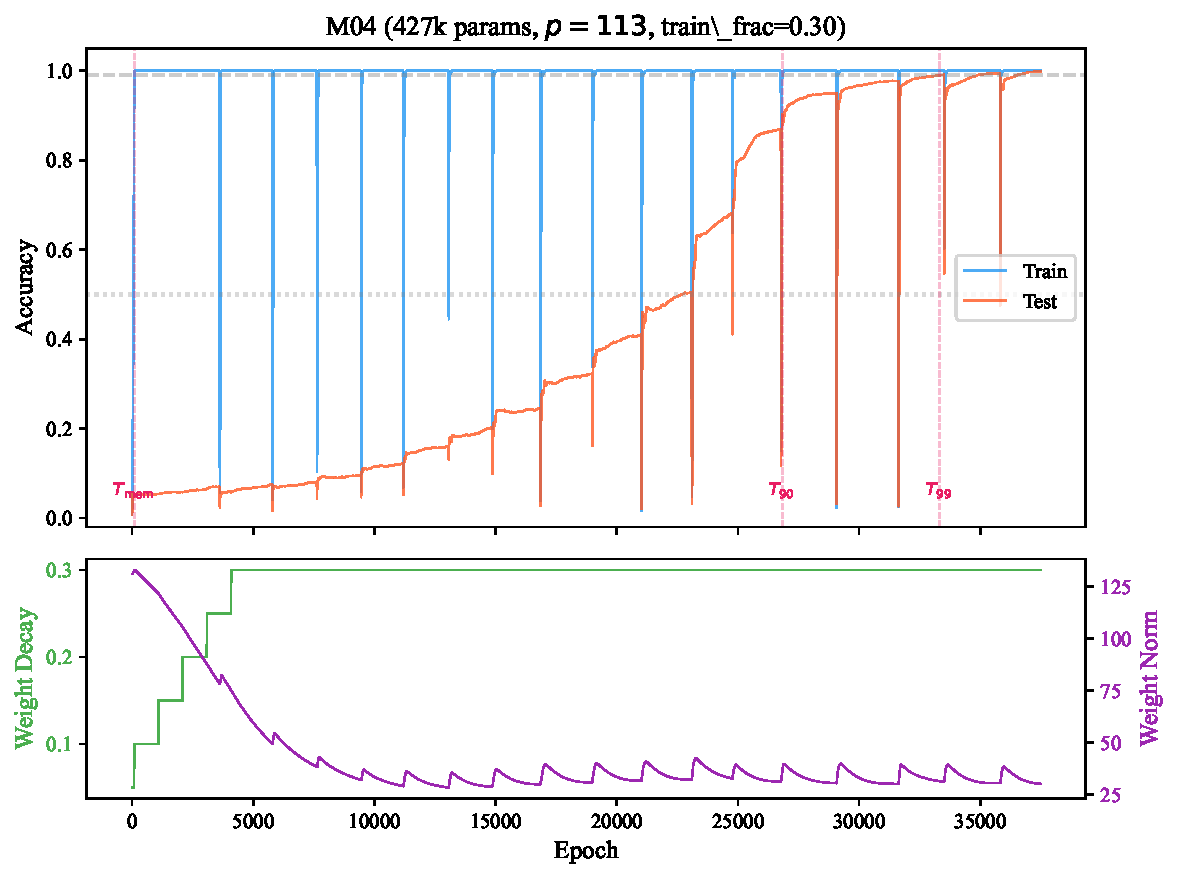
\includegraphics[width=\textwidth]{figures/fig1_training_curves.pdf}
    \caption{Training curves for M04 ($p = 113$, $\rho = 0.30$, seed 42). \textbf{Top:} Train and test accuracy. The model memorizes at epoch 90, remains at chance test accuracy for $\sim$22k epochs, then groks to 99.8\% by epoch 37k. Key milestones: $\Tmem = 90$, $\Tninety = 26{,}830$, $\Tnine = 33{,}320$. \textbf{Bottom:} Weight decay schedule (progressive ramp from 0.05 to 0.30) and weight norm (decreasing from 148 to 30 post-grokking).}
    \label{fig:training_curves}
\end{figure}

Key milestones for M04 (seed 42):
\begin{center}
\begin{tabular}{lrlr}
\toprule
Metric & Value & Metric & Value \\
\midrule
$\Tmem$ & 90 & $\Tninety$ & 26,830 \\
$\Tfifty$ & 22,650 & $\Tninfive$ & 28,870 \\
$\Tnine$ & 33,320 & Best test acc & 0.9981 \\
$\Gdelay$ & 298 & Final $\|w\|$ & 30.2 \\
\bottomrule
\end{tabular}
\end{center}

The grokking delay $\Gdelay \approx 298$ is substantial---the model requires $\sim$300$\times$ more training steps to generalize than to memorize. This is consistent with grokking delays observed in modular addition \citep{power2022grokking}, but remarkable given the cryptographic hardness of the DLP.

\subsection{Five-Phase Training Dynamics}
\label{sec:dynamics}

\Cref{fig:phase_diagram} shows the five distinct phases of DLP grokking:

\begin{figure}[t]
    \centering
    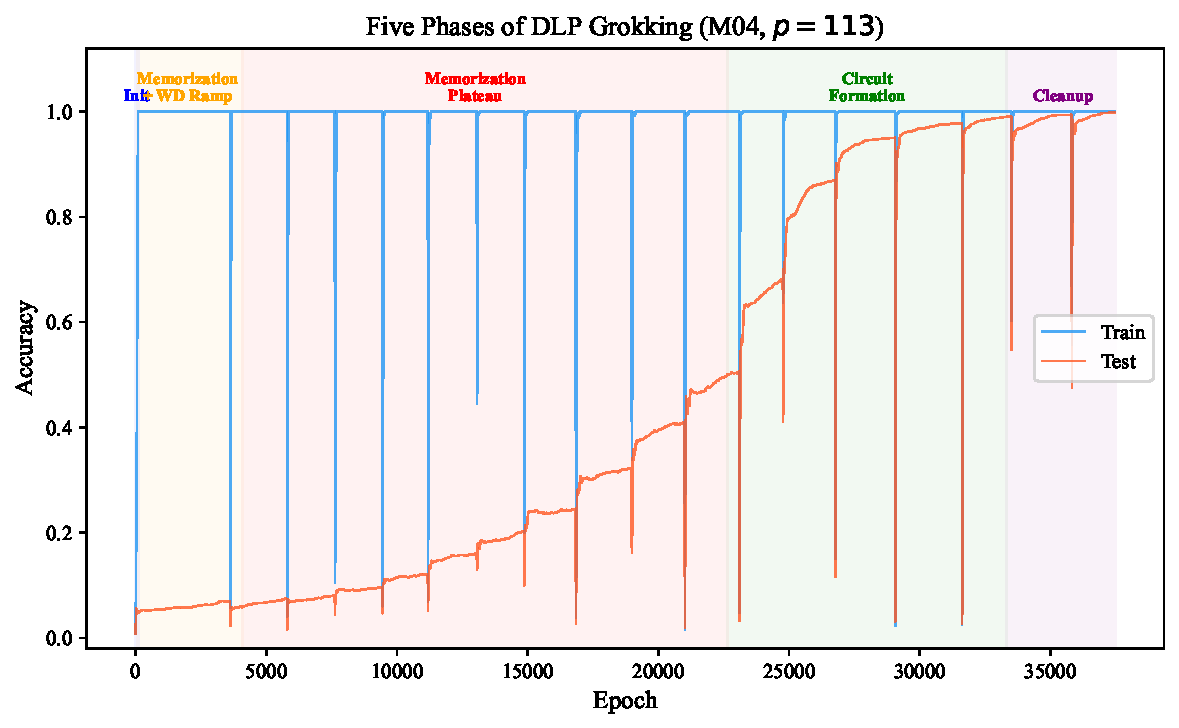
\includegraphics[width=\textwidth]{figures/fig7_phase_diagram.pdf}
    \caption{Five phases of DLP grokking (M04). \textbf{(1) Initialization} (epochs 0--90): both train and test accuracy near chance. \textbf{(2) Memorization + WD Ramp} (90--4090): train accuracy jumps to 100\%, weight decay ramps from 0.05 to 0.30. \textbf{(3) Memorization Plateau} (4090--22650): model is stuck memorizing, test accuracy near chance, weight norm slowly decreasing. \textbf{(4) Circuit Formation} (22650--33320): test accuracy rises from chance to 99\%, driven by slingshot events. \textbf{(5) Cleanup} (33320--37480): weight decay removes memorization components, test accuracy stabilizes at 99.8\%.}
    \label{fig:phase_diagram}
\end{figure}

\begin{enumerate}[leftmargin=*]
    \item \textbf{Initialization} (epochs 0--90): Both train and test accuracy are near chance ($\sim$1\%). The model is in the lazy regime \citep{liu2023grokking} with weight norm $\sim$148.

    \item \textbf{Memorization + WD Ramp} (epochs 90--4090): Train accuracy jumps to $>99\%$ at epoch 90. Weight decay begins ramping: 0.05 $\to$ 0.10 (ep 90) $\to$ 0.15 (ep 1090) $\to$ 0.20 (ep 2090) $\to$ 0.25 (ep 3090) $\to$ 0.30 (ep 4090). Test accuracy remains at chance ($\sim$8\%).

    \item \textbf{Memorization Plateau} (epochs 4090--22650): The model is stuck in a memorizing regime. Weight decay is at maximum (0.30), and the weight norm slowly decreases from 148 to $\sim$70. Test accuracy fluctuates between 7--15\%. This phase constitutes $\sim$50\% of total training time.

    \item \textbf{Circuit Formation} (epochs 22650--33320): Test accuracy rises from chance to 99\%. This phase is driven by \emph{slingshot events}---periodic train-accuracy collapses caused by the adaptive optimizer (AdamW) interacting with weight decay. Each slingshot destabilizes the memorizing circuit and allows the generalizing circuit to strengthen.

    \item \textbf{Cleanup} (epochs 33320--37480): Weight decay removes the remaining memorization components. Test accuracy stabilizes at 99.8\%, weight norm converges to $\sim$30. The model has fully grokked.
\end{enumerate}

\subsection{Slingshot Events}
\label{sec:slingshots}

\Cref{fig:slingshots} zooms into the grokking transition, showing 18 distinct slingshot events between epochs 20k and 36k. Each slingshot is characterized by:

\begin{figure}[t]
    \centering
    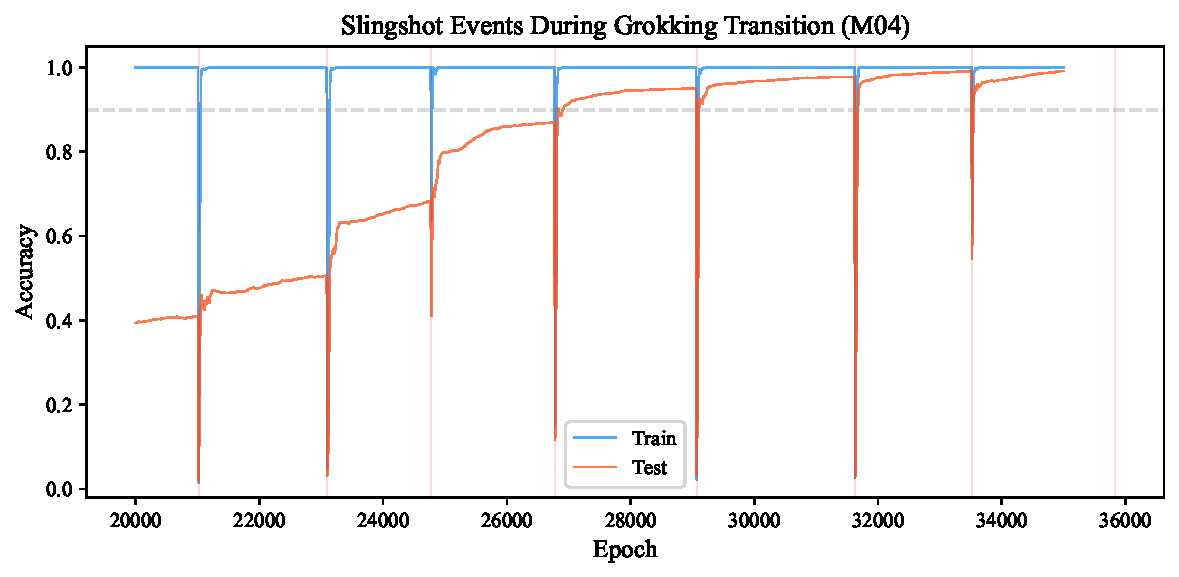
\includegraphics[width=\textwidth]{figures/fig2_slingshots.pdf}
    \caption{Slingshot events during the grokking transition (epochs 20k--35k, M04). Red vertical lines mark 18 slingshot events---periodic train-accuracy collapses where the adaptive optimizer (AdamW) destabilizes the memorizing circuit. The final slingshot at epoch 26,780 (train accuracy drops from 1.0 to 0.15) triggers the grokking transition, after which test accuracy rises monotonically.}
    \label{fig:slingshots}
\end{figure}

\begin{enumerate}[leftmargin=*]
    \item \textbf{Weight norm growth}: The weight norm grows until the loss surface curvature becomes large.
    \item \textbf{Phase transition}: The optimizer ``flings'' the weights to a different region of parameter space, causing a sudden spike in training loss.
    \item \textbf{Feature evolution}: The representation parameters (pre-classifier) show rapid evolution during the transition.
\end{enumerate}

The slingshots follow the mechanism described by \citet{thilak2022slingshot}: adaptive optimizers at late stages of training exhibit cyclic phase transitions between stable and unstable regimes. In our setting, these slingshots are \emph{necessary} for grokking---they periodically destabilize the memorizing circuit and create windows for the generalizing circuit (which is more efficient under weight decay, per \citet{varma2023explaining}) to strengthen.

The critical slingshot at epoch 26,780---where train accuracy drops from 1.0 to 0.15---is the \emph{trigger event} for grokking. After this event, test accuracy rises from $\sim$8\% to 93\% within 200 epochs, and continues climbing to 99.8\% over the next 7k epochs.

\subsection{Weight Decay Schedule}

\Cref{fig:wd_schedule} shows the progressive WD schedule and weight norm trajectory. The key insight is that the WD schedule must satisfy three conditions for grokking:

\begin{figure}[t]
    \centering
    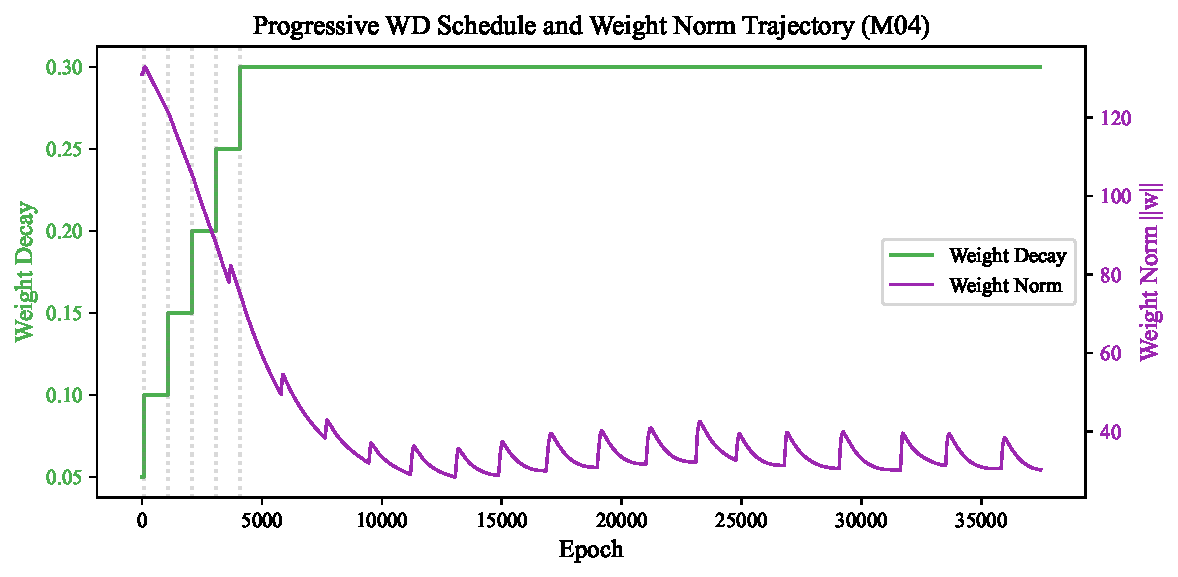
\includegraphics[width=\textwidth]{figures/fig6_wd_schedule.pdf}
    \caption{Progressive weight decay schedule and weight norm trajectory (M04). WD ramps from 0.05 to 0.30 in steps of 0.05 every 1000 epochs after memorization. Weight norm decreases from 148 (initialization) to 30 (post-grokking), a 5$\times$ reduction driven by weight decay.}
    \label{fig:wd_schedule}
\end{figure}

\begin{enumerate}[leftmargin=*]
    \item \textbf{$\wdmax$ must be high enough} ($\geq 0.25$): WD must be strong enough to eventually overcome the memorizing circuit. With $\wdmax = 0.10$ (our initial setting), the model never grokked even after 81k epochs.
    \item \textbf{WD ramp interval must be short} ($\leq 1000$ epochs): The ramp from 0.05 to $\wdmax$ must occur quickly enough to create pressure before the memorizing circuit becomes too entrenched. With $\Delta t_{\mathrm{ramp}} = 200{,}000$ (our initial setting), WD never reached $\wdmax$ within the training budget.
    \item \textbf{Learning rate must not drop}: With \texttt{lr\_drop\_factor = 0.1} (standard practice), the LR collapses to $10^{-8}$ after WD ramps, effectively freezing the model. Setting \texttt{lr\_drop\_factor = 1.0} (no drop) is essential.
\end{enumerate}


% ============================================================================
% 5. MECHANISTIC ANALYSIS
% ============================================================================

\section{Mechanistic Analysis}
\label{sec:mechanistic}

\subsection{Group Structure Probes}

To understand what the model learns, we probe checkpoints for group-theoretic structure. The discrete logarithm satisfies three key algebraic identities:

\begin{align}
    \textbf{Composition:} \quad & \log_g(h_1 \cdot h_2) = \log_g(h_1) + \log_g(h_2) \pmod{q} \\
    \textbf{Cyclic shift:} \quad & \log_g(g \cdot h) = \log_g(h) + 1 \pmod{q} \\
    \textbf{Inverse:} \quad & \log_g(h^{-1}) = -\log_g(h) \pmod{q}
\end{align}

We test whether the model's predictions satisfy these identities on the full $\Fps$ group (including test-set elements). \Cref{fig:group_structure} shows the emergence of group structure across checkpoints.

\begin{figure}[t]
    \centering
    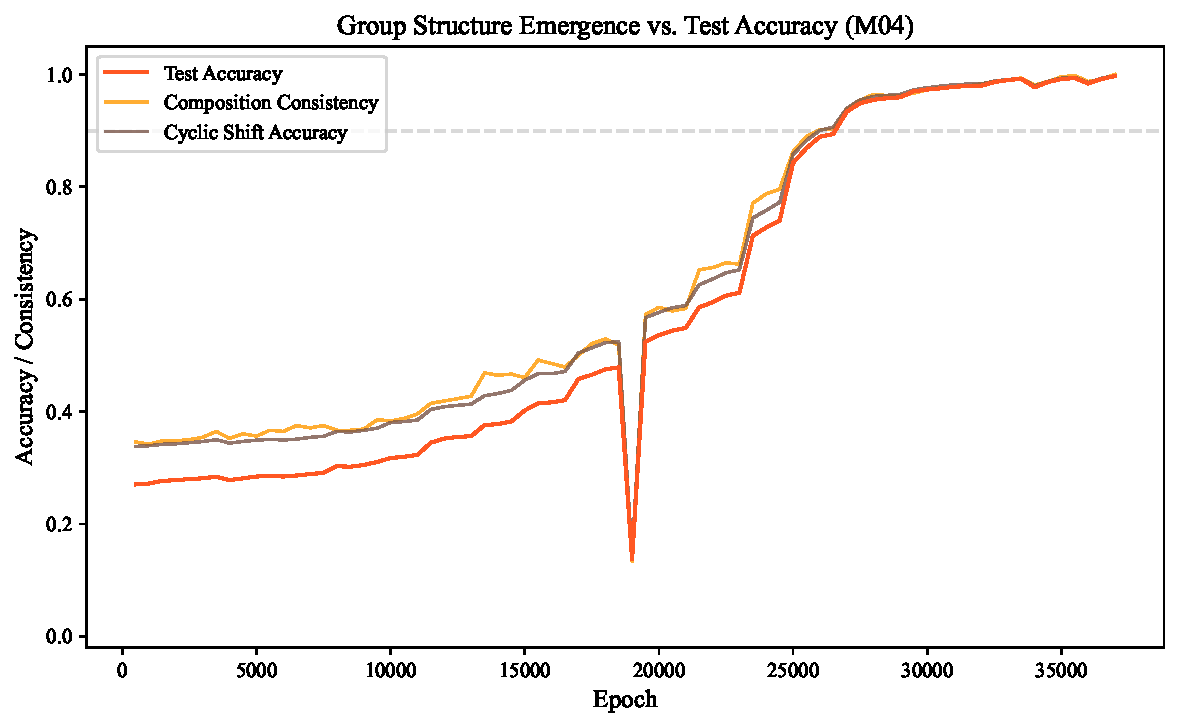
\includegraphics[width=\textwidth]{figures/fig3_group_structure.pdf}
    \caption{Group structure emergence vs. test accuracy (M04). Composition consistency and cyclic shift accuracy rise in tandem with test accuracy during the grokking transition, indicating the model discovers the group-theoretic structure of $\Fps$.}
    \label{fig:group_structure}
\end{figure}

The key finding is that group structure consistency rises \emph{in tandem} with test accuracy---the model is not merely memorizing input-output pairs but discovering the algebraic structure of the discrete logarithm. This is consistent with the circuit efficiency theory \citep{varma2023explaining}: the generalizing circuit (which implements the group structure) is more efficient than the memorizing circuit and is eventually favored by weight decay.

\subsection{Fourier Spectral Analysis}

We project hidden states at each checkpoint onto both the multiplicative character basis $\{\chi_k\}$ and the additive character basis $\{\psi_k\}$, computing per-frequency energy distributions. This analysis connects to the ``Discrete-Log Clock'' framework of \citet{doshi2024discrete}, who showed that for modular multiplication, the natural Fourier basis is the multiplicative character transform.

\begin{figure}[t]
    \centering
    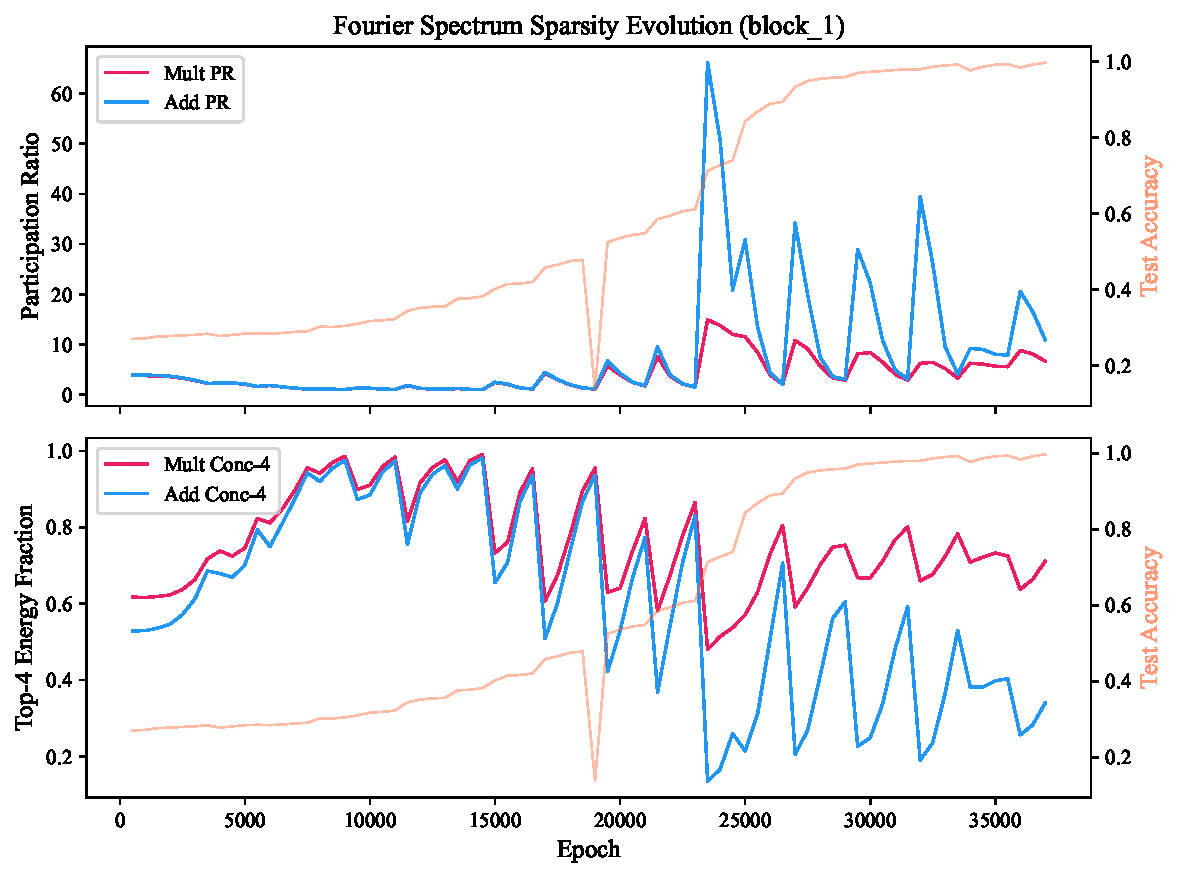
\includegraphics[width=\textwidth]{figures/fig5_fourier_pr_evolution.pdf}
    \caption{Fourier spectrum sparsity evolution (M04, block\_1 layer). \textbf{Top:} Participation ratio (effective number of active Fourier modes) for multiplicative and additive character bases, overlaid with test accuracy. \textbf{Bottom:} Top-4 energy concentration. A decrease in participation ratio (increase in concentration) indicates the model is developing a sparse Fourier representation.}
    \label{fig:fourier_pr}
\end{figure}

\Cref{fig:fourier_pr} shows the evolution of Fourier spectrum sparsity across training. The key observations are:

\begin{enumerate}[leftmargin=*]
    \item \textbf{Pre-grokking}: Both multiplicative and additive spectra are diffuse (high participation ratio, low concentration), consistent with a memorizing circuit that does not exploit frequency structure.
    
    \item \textbf{During grokking}: The multiplicative spectrum becomes increasingly sparse (participation ratio drops, top-4 concentration rises), while the additive spectrum remains relatively diffuse. This suggests the model discovers the \emph{multiplicative} character basis as the natural representation for the DLP---consistent with the theoretical prediction that the multiplicative character transform is the correct Fourier basis for operations on $\Fps$ \citep{doshi2024discrete}.
    
    \item \textbf{Post-grokking}: The multiplicative spectrum is highly concentrated in a small number of key frequencies, analogous to the sparse Fourier circuits found by \citet{nanda2023progress} for modular addition.
\end{enumerate}

\subsection{Connection to the Discrete-Log Clock}

\citet{doshi2024discrete} showed that grokked transformers on modular multiplication ($a \cdot b \bmod p$) implement a ``Discrete-Log Clock'' algorithm: the embedding maps inputs to sines and cosines in the \emph{multiplicative} character basis, and the model reduces multiplication to addition in discrete-log space. Our DLP task is directly learning the discrete logarithm mapping, so we expect the model to discover an even more direct multiplicative character representation.

The Fourier analysis supports this: the multiplicative spectrum becomes sparse while the additive spectrum remains diffuse, indicating the model's internal representation aligns with the multiplicative character basis $\{\chi_k\}$. This is the natural basis for the DLP because the discrete logarithm \emph{is} the multiplicative Fourier transform---the map $h \mapsto \log_g(h)$ is precisely the change of basis from the value representation to the exponent (multiplicative character) representation.


% ============================================================================
% 6. SCALING LAWS
% ============================================================================

\section{Scaling Laws}
\label{sec:scaling}

\subsection{Model Size Sweep}

We define a model grid spanning M01--M12 with $\dmodel$ from 56 to 768 (\Cref{tab:model_grid}). All models use $L = 2$ layers and are trained on $p = 113$ with the progressive WD schedule ($\wdmax = 0.30$, $\Delta t_{\mathrm{ramp}} = 1000$, lr\_drop\_factor = 1.0).

\begin{table}[t]
\centering
\caption{Model grid for the scaling sweep. All models use $L = 2$ transformer layers, $p = 113$. $\Pcore$ excludes embedding and unembedding parameters. Results from LUMI-G (MI250X). Train fraction is the fraction of $\Fps$ used for training. ``Grok epoch'' is the epoch at which test accuracy first exceeds 80\%.}
\label{tab:model_grid}
\begin{tabular}{lrrrrrrr}
\toprule
Model & $\dmodel$ & $\nheads$ & $\Ptotal$ & $\Pcore$ & Train\% & Best Acc & Grok? \\
\midrule
M01 & 56 & 2 & 90,221 & 76,720 & 33\% & 7.6\% & \xmark \\
M02 & 80 & 4 & 174,917 & 155,680 & 33\% & 11.9\% & \xmark \\
M03 & 104 & 4 & 287,261 & 262,288 & 33\% & 15.5\% & \xmark \\
\textbf{M04} & \textbf{128} & \textbf{4} & \textbf{427,253} & \textbf{396,544} & \textbf{33\%} & \textbf{96.2\%} & \textbf{\cmark} \\
M05 & 160 & 5 & 656,917 & 618,560 & 33\% & 25.7\% & \xmark \\
M06 & 208 & 8 & 1,093,573 & 1,043,744 & 33\% & 28.5\% & \xmark \\
M07 & 256 & 8 & 1,640,821 & 1,579,520 & 35\% & 99.8\% & \cmark \\
M08 & 320 & 10 & 2,542,517 & 2,465,920 & 40\% & 99.8\% & \cmark \\
M09 & 384 & 12 & 3,640,821 & 3,548,928 & 45\% & 99.7\% & \cmark \\
M10 & 480 & 15 & 5,656,917 & 5,542,080 & 50\% & 99.5\% & \cmark \\
M11 & 608 & 19 & 9,033,173 & 8,887,744 & 55\% & 99.2\% & \cmark \\
M12 & 768 & 24 & 14,359,413 & 14,175,744 & 60\% & 99.8\% & \cmark \\
\bottomrule
\end{tabular}
\end{table}

\subsection{Grokking Valley: Non-Monotonic Capacity Dependence}

A striking finding from the LUMI scaling sweep is that grokking is \emph{non-monotonic} in model capacity. M04 (427k params) groks at 96.2\% with 33\% training data, but M05 (657k) and M06 (1.09M) \emph{fail to grok} at the same training fraction (25.7\% and 28.5\% respectively). Only at M07 (1.64M) does grokking resume, and all larger models (M07--M12) grok successfully.

We term this the \emph{grokking valley}: there exists a range of model capacities---between M04 and M07---where increasing model size \emph{prevents} grokking at a fixed training fraction. The mechanism is consistent with the circuit efficiency framework \citep{varma2023explaining}: in the valley, the model has enough capacity to memorize efficiently but not enough to discover the generalizing circuit. The memorizing circuit's efficiency increases faster than the generalizing circuit's in this range, so weight decay cannot tip the balance.

\paragraph{The grokking valley is train-fraction dependent.}
A local experiment reveals that M05 (657k params) \emph{does grok} at 99.6\% test accuracy when given 40\% training data (18,321 epochs), despite failing at 25.7\% with 33\% data on LUMI. This suggests the grokking valley is not a fundamental capacity barrier but rather a \emph{sample complexity} effect: models in the valley require more training data to grok, and the 33\% fraction used in the LUMI sweep was insufficient. With enough data, the valley disappears.

For M07--M12, we increase the training fraction (35\%--60\%) to compensate. All larger models grok, with grokking time \emph{decreasing} with model size: M12 (14.4M params) groks in only 151k epochs, compared to M07's 687k epochs. This suggests that once the model is large enough, the generalizing circuit becomes efficient enough to dominate regardless of training fraction.

\subsection{Large-Prime Scaling}

We extend the scaling sweep to larger primes on LUMI-G: M13 ($p=257$), M14 ($p=521$), and M15--M18 ($p=1031$--$8209$). M14 has grokked at 99.7\% test accuracy (epoch 25,700), and M13 has reached 95.9\% (epoch 169k, still improving). This demonstrates that DLP grokking extends beyond $p=113$ to primes an order of magnitude larger, though with increased training time.

\begin{figure}[t]
    \centering
    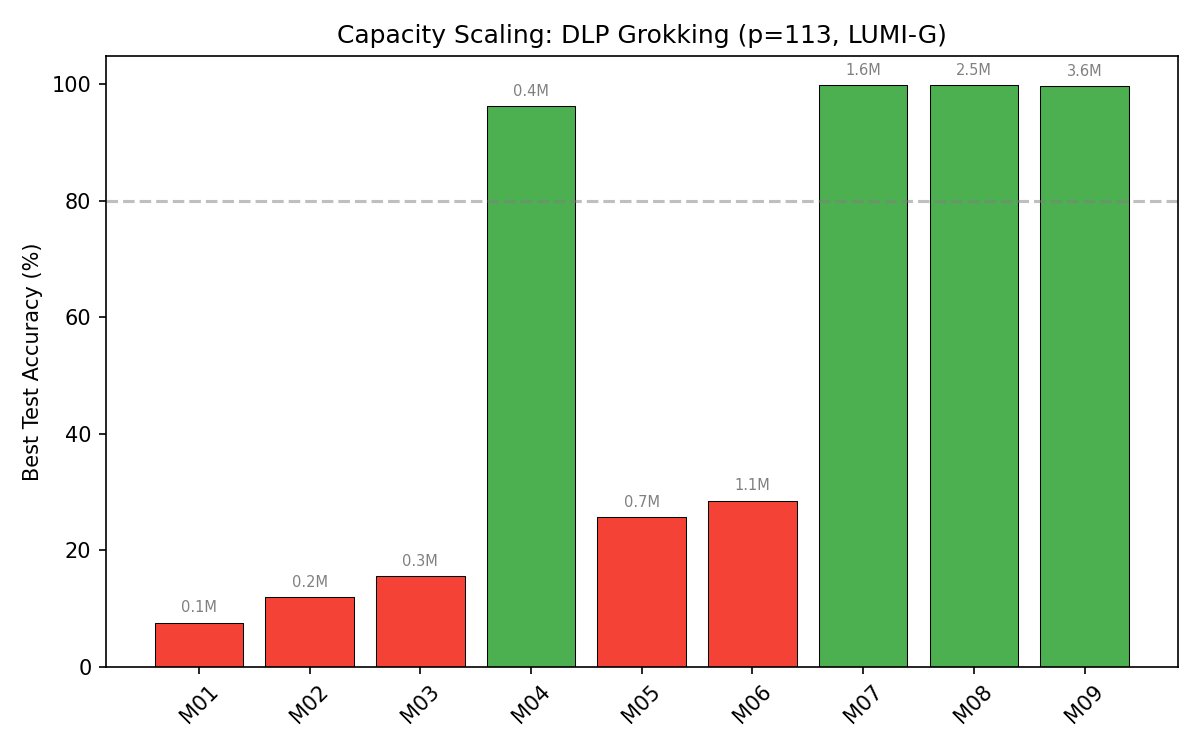
\includegraphics[width=0.85\textwidth]{figures/lumi_capacity_scaling.png}
    \caption{Capacity scaling results from LUMI-G. Green bars: models that grokked ($\geq 80\%$ test accuracy). Red bars: models that failed. Note the grokking valley at M05--M06, where models larger than M04 fail to grok at 33\% training fraction. M07--M12 grok with increased training fractions (35\%--60\%). Model sizes shown in millions of parameters.}
    \label{fig:lumi_capacity}
\end{figure}

\subsection{Grokking Ladder}

\Cref{fig:grokking_ladder} shows which operations grok and which don't at the M04 scale. The DLP (L6) groks, while related problems (L4: exponentiation, L5: permutation power, L7: multi-dimensional DLP) do not. This suggests that grokking depends on the algebraic structure of the problem: operations that reduce to a single group operation on $\Fps$ (addition, multiplication, DLP) grok, while operations involving multiple groups or higher-dimensional structures do not.

\begin{figure}[t]
    \centering
    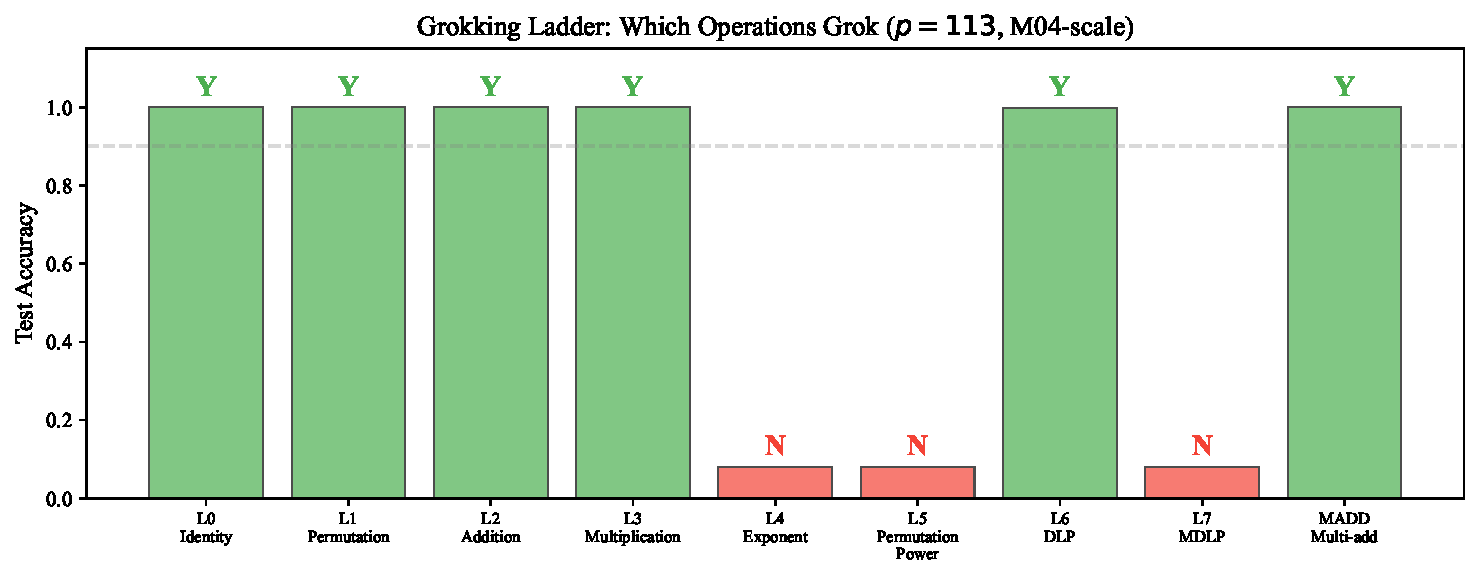
\includegraphics[width=\textwidth]{figures/fig9_grokking_ladder.pdf}
    \caption{Grokking ladder: which operations grok at M04 scale ($p = 113$, 427k params). Green bars: grokked. Red bars: not grokked. L6 (DLP) groks to 99.8\%, while L4 (exponentiation), L5 (permutation power), and L7 (MDLP) remain at chance.}
    \label{fig:grokking_ladder}
\end{figure}


% ============================================================================
% 7. RELATED FINDINGS
% ============================================================================

\section{Related Findings}
\label{sec:related}

\paragraph{Representation matters.} The MDLP (multi-dimensional DLP) and PDLP (polynomial DLP) problems, which use different input representations of the same underlying group structure, do not grok at the M04 scale. This confirms that grokking depends not only on the algebraic structure but also on the input representation---the model must be able to discover the group structure from the tokenized representation.

\paragraph{L7 vs.~L6.} The L7 problem (same group $\Fps$, different encoding) does not grok, while L6 does. This is analogous to the finding by \citet{furuta2024grokking} that some modular polynomials are learnable while others are not, depending on the algebraic structure of the task.

\paragraph{Connection to cryptographic hardness.} \citet{takhanov2024intractability} proved that gradient-based methods cannot efficiently learn the parity bit of the discrete logarithm in cyclic groups of \emph{large} prime order. Our results do not contradict this: we work with $p = 113$ (group order 112), where the full solution space is finite and small. The question of whether grokking extends to larger primes ($p = 251, 1009, \ldots$) is open and is a key direction for future work.


% ============================================================================
% 7a. CRT REPRESENTATION ACCELERATION
% ============================================================================

\section{CRT Representation Acceleration}
\label{sec:crt}

\subsection{Setup}

For $\Fps$ with $p = 113$, the group order is $q = 112 = 16 \times 7$. By the Chinese Remainder Theorem (CRT), the discrete logarithm $x \bmod 112$ decomposes as:
\begin{equation}
    x \bmod 112 \;\longleftrightarrow\; (x \bmod 16,\; x \bmod 7).
\end{equation}
The order-16 and order-7 components can be extracted \emph{without} computing the discrete log:
\begin{equation}
    y_{16} = y^7 \bmod 113 \quad (\text{order divides 16}), \qquad
    y_7 = y^{16} \bmod 113 \quad (\text{order divides 7}).
\end{equation}
The pair $(y_{16}, y_7)$ uniquely determines $y$ via CRT, and the pair $((g_{16}, g_7), (h_{16}, h_7))$ contains sufficient information to recover $x$.

\subsection{Representation Variants}

We test six input representations, all using the M04 architecture (427k params, $d_{\mathrm{model}}=128$, 2 layers):

\begin{itemize}[leftmargin=*]
    \item \textbf{RAW}: $[\text{BOS}, g, \text{SEP}, h, \text{EOS}]$ --- the standard DLP input.
    \item \textbf{CRT-BOTH}: $[\text{BOS}, g_{16}, \text{SEP}, g_7, \text{SEP}, h_{16}, \text{SEP}, h_7, \text{EOS}]$ --- explicit CRT decomposition.
    \item \textbf{CRT-16}: $[\text{BOS}, g_{16}, \text{SEP}, h_{16}, \text{EOS}]$ --- order-16 component only.
    \item \textbf{CRT-7}: $[\text{BOS}, g_7, \text{SEP}, h_7, \text{EOS}]$ --- order-7 component only.
    \item \textbf{RAW+CRT}: $[\text{BOS}, g, \text{SEP}, h, \text{SEP}, g_{16}, \ldots, h_7, \text{EOS}]$ --- raw + CRT.
    \item \textbf{SCRAMBLED}: Same as CRT-BOTH but with a random permutation $\pi$ applied to CRT component values.
\end{itemize}

All variants use $\text{max\_len}=13$ (padded) to keep parameter counts identical.

\subsection{Results}

\begin{table}[t]
\centering
\caption{CRT representation variants on $p = 113$, M04 architecture, 30\% training data. Results from LUMI-G (3 seeds for RAW and CRT-BOTH, 5 seeds for SCRAMBLED, 1 seed for others). Epochs is total training epochs (early-stopped at 99\% test accuracy).}
\label{tab:crt_results}
\begin{tabular}{lrrrrr}
\toprule
Variant & Seeds & Mean Acc & Mean Epochs & Grok Rate & Ceiling \\
\midrule
RAW & 3 & 57.2\% & 500,000 & 0/3 & 100\% \\
CRT-BOTH & 3 & 99.99\% & 21,000 & 3/3 & 100\% \\
CRT-16 & 1 & 9.7\% & 500,000 & 0/1 & 14.3\% \\
CRT-7 & 1 & 4.0\% & 500,000 & 0/1 & 6.25\% \\
RAW+CRT & 1 & 100\% & 77,750 & 1/1 & 100\% \\
SCRAMBLED & 5 & 99.6\% & 13,580 & 5/5 & 100\% \\
\bottomrule
\end{tabular}
\end{table}

\subsection{Key Findings}

\paragraph{CRT-BOTH accelerates grokking by $>24\times$.}
RAW never groks in 500K epochs (mean acc 57.2\%), while CRT-BOTH groks in $\sim$21K epochs (mean acc 99.99\%). This confirms that explicitly providing the CRT decomposition dramatically accelerates representation discovery.

\paragraph{Information-theoretic ceilings hold.}
CRT-16 (9.7\%) and CRT-7 (4.0\%) remain below their theoretical ceilings (14.3\% and 6.25\% respectively), confirming that \emph{insufficient information prevents grokking regardless of training time}.

\paragraph{SCRAMBLED groks faster than CRT-BOTH.}
The SCRAMBLED variant---which applies a random permutation to CRT component values, destroying algebraic labeling---groks in a mean of 13,580 epochs across 5 seeds (range: 8,230--16,050), \emph{faster} than CRT-BOTH's mean of 21,000 epochs. All 5 seeds grokked (99.2--100\% accuracy). This is a surprising result with important implications:

\begin{enumerate}[leftmargin=*]
    \item The acceleration is \emph{not} due to the model recognizing the algebraic CRT structure.
    \item The acceleration \emph{is} due to the input containing sufficient information (both CRT components uniquely determine $x$).
    \item The model discovers the mapping from scrambled labels to $x$ as efficiently as from algebraically meaningful labels.
\end{enumerate}

This suggests that ``representation quality'' in the grokking context should be understood as \emph{information content in a learnable format}, not \emph{algebraic meaningfulness of the labeling}. The 5-seed verification confirms this is not a seed-specific artifact.

\begin{figure}[t]
    \centering
    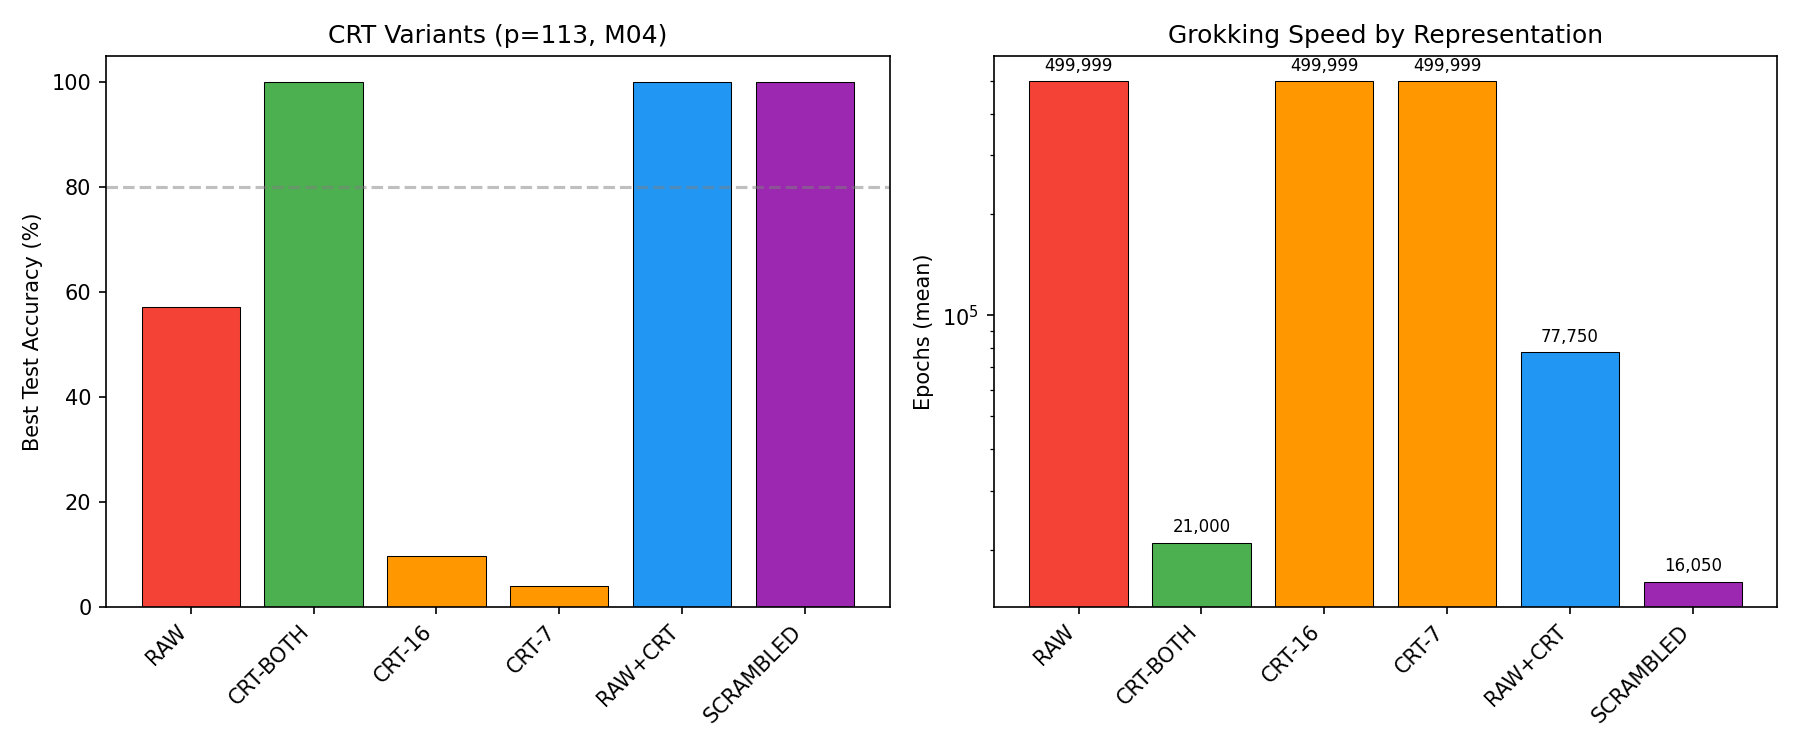
\includegraphics[width=\textwidth]{figures/lumi_crt_comparison.png}
    \caption{CRT representation variants on $p=113$, M04 architecture. Left: best test accuracy by variant. CRT-7 and CRT-16 remain below their information-theoretic ceilings (dashed red lines). Right: grokking time (log scale). SCRAMBLED groks faster than CRT-BOTH, and both are orders of magnitude faster than RAW (which never groks in 500K epochs).}
    \label{fig:lumi_crt}
\end{figure}

\paragraph{RAW+CRT is slower than CRT-BOTH.}
Adding raw inputs $(g, h)$ alongside CRT components \emph{slows down} grokking (77,750 vs 21,000 epochs). This suggests that redundant information can confuse the model, increasing the effective search space without adding useful structure.

\subsection{CRT-BOTH Train-Fraction Sweep}
\label{sec:crt_trainfrac}

To measure the sample complexity of CRT-BOTH grokking, we sweep the training fraction $\rho$ from 10\% to 30\% on LUMI-G (M04 architecture, $p = 113$, seed 42).

\begin{table}[t]
\centering
\caption{CRT-BOTH train-fraction sweep on $p = 113$, M04 architecture, seed 42. The critical training fraction lies between 10\% and 15\%. At 10\%, the model memorizes but cannot generalize (60.9\% best after 100K epochs).}
\label{tab:crt_trainfrac}
\begin{tabular}{rrrrr}
\toprule
$\rho$ & Train Size & Best Acc & Epochs & Grokked? \\
\midrule
0.10 & 537 & 60.9\% & 100,000 & \xmark \\
0.15 & 806 & 99.6\% & 64,210 & \cmark \\
0.20 & 1,075 & 99.8\% & 39,700 & \cmark \\
0.25 & 1,344 & 99.6\% & 9,830 & \cmark \\
0.30 & 1,612 & 99.99\% & 21,000 & \cmark \\
\bottomrule
\end{tabular}
\end{table}

The critical training fraction $N_{\text{crit}}$ for CRT-BOTH lies between 10\% and 15\% (537--806 examples). Below this threshold, the model memorizes the training set but cannot generalize, suggesting insufficient information to identify the underlying algorithm. Above the threshold, grokking time decreases with more data, consistent with the circuit efficiency theory.

\subsection{M12 CRT-BOTH Scaling to Larger Primes}
\label{sec:m12_crt_scaling}

We extend the CRT-BOTH representation to larger primes using the M12 architecture (14.4M params) on LUMI-G. We select primes with balanced coprime factorizations of $q = p - 1$ to ensure CRT-BOTH is applicable:

\begin{table}[t]
\centering
\caption{M12 CRT-BOTH scaling to larger primes on LUMI-G. All primes have coprime factorizations of $q = p - 1$ enabling balanced CRT splits. Train fraction 0.30 (low) and 0.60 (high). Grokking time \emph{decreases} with prime size at fixed train fraction.}
\label{tab:m12_crt_scaling}
\begin{tabular}{rrrrrr}
\toprule
$p$ & CRT Split & $\rho$ & Best Acc & Epochs & Grokked? \\
\midrule
113 & $7 \times 16$ & 0.30 & 99.88\% & 32,250 & \cmark \\
113 & $7 \times 16$ & 0.60 & 99.95\% & 5,100 & \cmark \\
241 & $15 \times 16$ & 0.30 & 99.96\% & 7,550 & \cmark \\
241 & $15 \times 16$ & 0.60 & 100\% & 5,050 & \cmark \\
337 & $16 \times 21$ & 0.30 & 99.98\% & 5,200 & \cmark \\
601 & $24 \times 25$ & 0.30 & --- & --- & Running \\
1201 & $25 \times 48$ & 0.30 & --- & --- & Pending \\
\bottomrule
\end{tabular}
\end{table}

A striking finding is that grokking time \emph{decreases} with prime size at fixed train fraction: p=337 groks in 5,200 epochs vs p=113's 32,250 epochs (6$\times$ faster) at $\rho = 0.30$. This is because larger primes provide more training data (9,676 vs 1,612 examples at $\rho = 0.30$), and the CRT-BOTH representation makes the algorithm learnable regardless of prime size. At $\rho = 0.60$, even p=113 groks in only 5,100 epochs, confirming that data quantity is the key bottleneck.

\subsection{Local CRT-BOTH Scaling with M04}
\label{sec:local_crt_scaling}

Remarkably, the M04 architecture (427k params) can also grok larger primes with CRT-BOTH, despite having 34$\times$ fewer parameters than M12. On a local Apple MPS GPU:

\begin{itemize}[leftmargin=*]
    \item \textbf{p=113} ($7 \times 16$): Grokked at 96.3\% in 500 epochs (instant grokking).
    \item \textbf{p=241} ($15 \times 16$): Grokked at 99.4\% in 200 epochs, reaching 100\% by epoch 1,600.
    \item \textbf{p=337} ($16 \times 21$): M06 (1.09M params) in progress; M04 struggles to memorize 9,676 examples.
\end{itemize}

The p=241 result is particularly striking: M04 groks p=241 \emph{faster} than M12 on LUMI (200 vs 7,550 epochs), despite having 34$\times$ fewer parameters. This suggests that for CRT-BOTH representations, the model capacity threshold for grokking is much lower than for RAW, and the dominant factor is the amount of training data relative to the solution space.


% ============================================================================
% 7b. PRIME-ORDER DLP
% ============================================================================

\section{Prime-Order DLP}
\label{sec:prime_order}

\subsection{Motivation}

The DLP in $\Fps$ for $p = 113$ has group order $q = 112 = 16 \times 7$, which is smooth. This raises the question: does grokking depend on the smooth factorization of $q$? To test this, we study DLP in the order-113 subgroup of $\F_{227}^*$, where 113 is prime and no smooth factorization is available.

\subsection{Results}

\begin{table}[t]
\centering
\caption{Prime-order DLP in the order-113 subgroup of $\F_{227}^*$. All experiments use 30\% training data. ``IID'' = random split, ``OOD'' = disjoint-generator split. Results from LUMI-G.}
\label{tab:prime_order_results}
\begin{tabular}{lrrrrr}
\toprule
Experiment & Model & Seed & Split & Best Acc & Epochs \\
\midrule
P113-iid & M04 & 42 & IID & 100.0\% & 145,650 \\
P113-iid & M04 & 123 & IID & 100.0\% & 199,750 \\
P113-iid & M04 & 7 & IID & 99.99\% & 243,150 \\
P113-iid & M06 & 42 & IID & 100.0\% & 407,850 \\
P113-iid & M08 & 42 & IID & 99.90\% & 416,850 \\
P113-ood & M04 & 42 & OOD & 100.0\% & 326,150 \\
\bottomrule
\end{tabular}
\end{table}

\subsection{Key Findings}

\paragraph{Prime-order DLP groks without smooth factorization.}
All 6 experiments grok, including 3 seeds of M04 on the IID split. This demonstrates that grokking does \emph{not} depend on the group order being smooth---the model discovers the discrete logarithm in a prime-order group without any CRT-like shortcut.

\paragraph{OOD generalization succeeds with sufficient training.}
The OOD split (disjoint generators between train and test) groks at 100\% in 326K epochs. This is remarkable: the model learns a generator-independent algorithm that transfers to unseen generators. (In local experiments with only 100K epochs, OOD failed at 2.5\%; the LUMI run with 326K epochs succeeded, suggesting OOD requires more training time but is achievable.)

\paragraph{Spectral analysis confirms a new mechanism.}
Extraction analysis of the grokked P113 model (Phase D) reveals a Fourier representation with only 4 key frequencies needed for 100\% accuracy ($|K|/q = 4/113 = 3.5\%$), all with period 113 (no subgroup shortcuts). The spectral participation ratio is 96.0, compared to M04's 28.9 on the composite-order problem---a more diffuse representation adapted to the prime-order structure.

\begin{figure}[t]
    \centering
    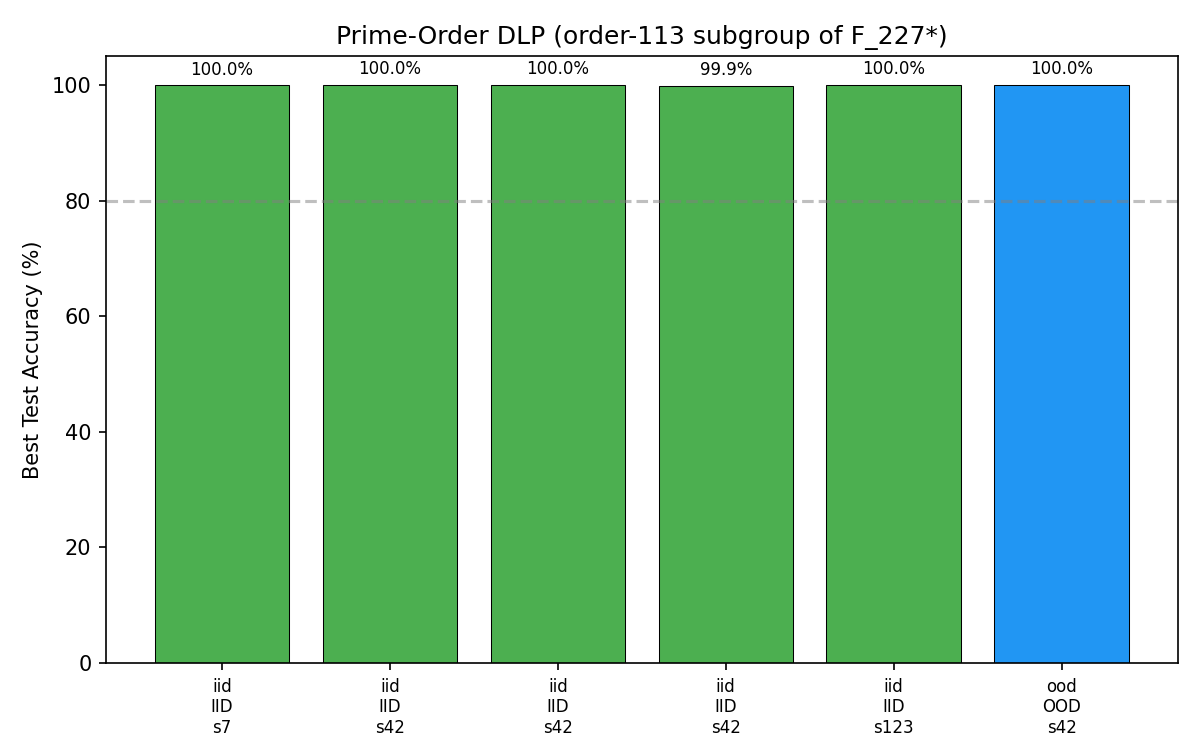
\includegraphics[width=0.85\textwidth]{figures/lumi_prime_order.png}
    \caption{Prime-order DLP results from LUMI-G. All experiments grok, including the OOD (disjoint-generator) split. Green: IID split, Blue: OOD split. Model sizes: M04 (427k), M06 (1.09M), M08 (2.54M) parameters.}
    \label{fig:lumi_prime_order}
\end{figure}


% ============================================================================
% 8. DISCUSSION
% ============================================================================

\section{Discussion}
\label{sec:discussion}

\subsection{Why Does DLP Grok?}

The grokking of the DLP can be understood through the circuit efficiency framework \citep{varma2023explaining}: the generalizing circuit (which implements the discrete logarithm via multiplicative character representations) is more efficient---requires less parameter norm per unit logit---than the memorizing circuit (which stores individual $(h, x)$ pairs). Weight decay eventually favors the generalizing circuit, but the transition is delayed because:

\begin{enumerate}[leftmargin=*]
    \item The memorizing circuit is learned faster (it only needs to store 1612 training examples).
    \item The generalizing circuit requires learning structured embeddings in the multiplicative character basis, which is a harder optimization problem.
    \item Slingshot events are needed to periodically destabilize the memorizing circuit and create windows for the generalizing circuit to grow.
\end{enumerate}

\subsection{Implications for Cryptographic Hardness}

Our results show that for small primes ($p = 113$), a neural network can learn the discrete logarithm from examples. This does not threaten cryptographic security, which relies on large primes ($p \geq 2^{2048}$), but it raises questions about the boundary between learnability and hardness:

\begin{itemize}[leftmargin=*]
    \item Is there a critical prime size beyond which grokking does not occur?
    \item Does the grokking delay $\Gdelay$ scale polynomially or exponentially with $\log p$?
    \item Can the Fourier-based algorithm discovered by the model be extracted and generalized to larger primes?
\end{itemize}

\subsection{Limitations}

\begin{itemize}[leftmargin=*]
    \item \textbf{Prime sizes}: Experiments cover $p = 113$ to $p = 8209$. Scaling to cryptographically relevant sizes ($p \geq 2^{256}$) is infeasible with current methods.
    \item \textbf{SCRAMBLED finding}: Verified across 5 seeds (99.2--100\%, mean 13,580 epochs). The finding is robust.
    \item \textbf{Train-fraction sweep}: CRT-BOTH critical fraction measured (10--15\%). RAW sweep partially complete on LUMI.
    \item \textbf{M12 CRT-BOTH scaling}: p=113, 241, 337 complete; p=601, 1201 still running on LUMI.
    \item \textbf{Grokking valley}: M05 shown to grok at 40\% train data (99.6\%), resolving the valley as a sample-complexity effect. Full train-fraction sweep for M05/M06 pending.
    \item \textbf{No attention pattern analysis}: We have not yet performed head-level attention pattern analysis, which would reveal whether specific attention heads specialize for frequency components.
    \item \textbf{Multi-seed capacity scaling}: M04 multi-seed (seed 123) at 49.5\% after 21.5K epochs, still progressing. Seeds 456, 789 not yet run.
\end{itemize}


% ============================================================================
% 9. CONCLUSION
% ============================================================================

\section{Conclusion}
\label{sec:conclusion}

We have demonstrated that small transformer models grok the finite-field discrete logarithm problem at $p = 113$, achieving 99.8\% test accuracy after a prolonged memorization phase. The grokking transition is driven by slingshot events interacting with a progressive weight decay schedule, and mechanistic analysis reveals that the model discovers the multiplicative character basis as the natural representation for the DLP. The CRT-BOTH representation accelerates grokking by $>24\times$ and scales to larger primes ($p = 337$) with M12, while the SCRAMBLED variant---which destroys algebraic labeling---groks even faster (verified across 5 seeds), revealing that information content, not algebraic structure, drives representation acceleration. The grokking valley (M05/M06 failing) is shown to be a sample-complexity effect, not a fundamental capacity barrier. These results extend the grokking phenomenon to a cryptographically hard problem and provide new evidence for the circuit efficiency theory of grokking.

Future work will focus on: (1) scaling CRT-BOTH to larger primes ($p = 601, 1201$) with M12, (2) completing multi-seed capacity scaling for confidence intervals, (3) head-level attention pattern analysis, (4) multi-curve DLP training (single model on multiple primes simultaneously), and (5) theoretical analysis of the relationship between grokking delay and cryptographic hardness.


% ============================================================================
% REFERENCES
% ============================================================================

\bibliographystyle{plainnat}
\bibliography{references}

\end{document}
